% --------------------------------------------------------------------------
% Template for IWAENC 2022 papers; to be used with:
%          spconfa4.sty  - ICASSP/ICIP LaTeX style file, and
%          IEEEbib.bst - IEEE bibliography style file.
%
% (Last modified by H. Loellmann, LMS, FAU Erlangen-Nuremberg, Jan. 2020)
%
% --------------------------------------------------------------------------

\documentclass{article}
\usepackage[preprint]{spconfa4}
\usepackage{amsmath,graphicx}
\usepackage[dvipsnames]{xcolor}
\usepackage{tikz}
\usetikzlibrary{arrows,snakes,backgrounds,matrix,patterns,positioning,fadings}
\usepackage{standalone}
\usepackage{subfig}
\usepackage{upgreek}
\usepackage{nicefrac}
\usepackage{dsfont}
\usepackage{bm}
\usepackage{cancel}
\usepackage{amsbsy}
\usepackage{algorithm}
\usepackage{algpseudocode}
\usepackage{lipsum}
\usepackage{harpoon}
\usepackage{comment}
\newenvironment{note}
 {\par\textcolor{Blue}{\bfseries Note:} \color{Blue}\ignorespaces}
 {\par}
\newenvironment{attention}
 {\par\textcolor{red}{\bfseries Attention:} \color{red}\ignorespaces}
 {\par}
\usepackage{hyperref}
\hypersetup{
	colorlinks,
	linkcolor={blue!80!black},
	citecolor={blue!80!black},
	urlcolor={blue!80!black}
}

\newcommand{\mtxb}[1]{\bm{\mathrm{#1}}}
\newcommand{\T}{{\mathrm{T}}}
\newcommand{\herm}{{\mathrm{H}}}
\newcommand{\ev}[1]{\mathrm{E} \left\lbrace #1 \right\rbrace}

% \excludecomment{note}
% \excludecomment{attention}

% Common variables
\newcommand{\h}{\mtxb{h}}
\newcommand{\x}{\mtxb{x}}
\newcommand{\R}{\mtxb{R}}
\newcommand{\w}{\mtxb{w}}
\newcommand{\z}{\mtxb{z}}
\newcommand{\uu}{\mtxb{u}}
\newcommand{\aRho}{\mtxb{P}}
\newcommand{\I}{\mtxb{I}}

% IMPORTANT: Add copyright notice by uncommenting the appropriate line
%----------------------------------------------------------
% For papers in which all authors are employed by the US government,
% \copyrightnotice{U.S. Government work not protected by U.S. copyright}

% For papers in which all authors are employed by a Crown government (UK, Canada, and Australia)
% \copyrightnotice{978-1-6654-6867-1/22/\$31.00~\copyright2022 Crown}
                   
% For papers in which all authors are employed by the European Union,
% \copyrightnotice{978-1-6654-6867-1/22/\$31.00~\copyright2022 European Union}
                   
% For all other papers the copyright notice is
\copyrightnotice{978-1-6654-6867-1/22/\$31.00~\copyright2022 IEEE}
                   
% Title.
% ------
\title{CROSS-RELATION BASED BLIND SYSTEM IDENTIFICATION USING ONLINE ADMM}
%
% Single address.
% ---------------
\name{Matthias Blochberger\sthanks{THANK EU!}, Filip Elvander\sthanks{THANK FWO?}, Randall Ali, Toon van Waterschoot}
\address{KU Leuven\\ESAT - Department of Electrical Engineering\\STADIUS\\3001 Leuven}
%
% For example:
% ------------
%\address{School\\
%	Department\\
%	Address}
%
% Two addresses (uncomment and modify for two-address case).
% ----------------------------------------------------------
%\twoauthors
%  {A. Author-one, B. Author-two\sthanks{Thanks to XYZ agency for funding.}}
%	{School A-B\\
%	Department A-B\\
%	Address A-B}
%  {C. Author-three, D. Author-four\sthanks{The fourth author performed the work
%	while at ...}}
%	{School C-D\\
%	Department C-D\\
%	Address C-D}
%
\begin{document}
%\ninept
%
\maketitle
%
\begin{abstract}
The abstract should appear at the top of the left-hand column of text, about 0.5 inch (12 mm) below the title area and no more than 3.125 inches (80 mm) in length.
Leave a 0.5 inch (12 mm) space between the end of the abstract and the beginning of the main text.
The abstract should contain about 100 to 150 words, and should be identical to the abstract text submitted electronically.
All manuscripts must be in English.
\end{abstract}
%
\begin{keywords}
blind system identification, multichannel signal processing, ADMM, Online-ADMM
\end{keywords}
%
\section{Introduction}
\label{sec:intro}

Its my pleasure to introduce to you: Algorithm. The most accurate, the fastest, the one most robust to noise; Simply the best you can get. Please give a warm welcome and a big applause!

% \lipsum[1-4]

% #############################################################################
% #############################################################################
\section{Problem statement}
\label{sec:problem_statement}


% #############################################################################
\subsection{Signal Model}
\label{ssec:signal_model}
We define the acoustic SIMO system with the input signal \(\mtxb{s}(n) = \begin{bmatrix}
    s(n)&s(k-1)&\cdots&s(k-2L+2)
\end{bmatrix}^{\T}\) and \(i \in [M]\) outputs 
\(
    \x_i(n) = \begin{bmatrix}
        x_i(n)&x_i(k-1)&\cdots&x_i(k-L+1)
    \end{bmatrix}^{\T}
\).
Each output \(\x_i\) is the convolution of \(\mtxb{s}\) with the respective channel impulse response \(\h_i\) with additive noise term \(\mtxb{v}_i\), assumed to be zero-mean and uncorrelated.
The signal model is described by
\begin{equation}
    \x_i(n) = \mtxb{H}_i \mtxb{s}(n) + \mtxb{v}_i(n)
\end{equation}
where \(\mtxb{H}_i\) is the \(L \times (2L-1)\) linear convolution matrix of the \(i\)th channel using the elements of \(\h_i\).
\begin{note}
    Add definition of \(\mtxb{H}_i\)? Will take a lot of space.
\end{note}

% #############################################################################
\subsection{Cross-relation approach}
\label{ssec:cross_rel}
The cross-relation approach for BSI \cite{} aims to only use output signals of the system to identify it.
This is achieved by exploiting the relative channel information when more than one system output are available and certain identifiability conditions are satisfied:
\begin{itemize}
    \item Condition 1
    \item Condition 2
\end{itemize}

\noindent The fundamental equality of this approach is 
\begin{equation}
    \x_i^{\T}(n) \h_j = \x_j^{\T}(n) \h_i,\quad i,j=1,2,...,M,\,i\neq j\label{eq:cross_rel:equality_conv}
\end{equation}
which states that the output signal of one channel convolved with the impulse response of another is equal to the vice-versa.
This follows from the commutative nature of the convolution operation.
Using the (estimated) covariance \(\R_{ij} = \ev{\x_i \x_j^\T}\) instead of the signal vectors \(\x_i\) yields a more convenient problem formulation.
For the subsequent explanations the time index is dropped to make notation more compact, however the variables are time-variant.

We can combine all cross-relations \eqref{eq:cross_rel:equality_conv} into a linear system of equations
\begin{equation}
    \R \h = \bm{0} \label{eq:cross_rel:null_space}\\
\end{equation}
where 
\begin{equation}
    \R = \begin{bmatrix}
        \sum_{m \neq 1} \R_{mm} & -\R_{21} & \cdots & -\R_{M1}\\
        -\R_{12} & \sum_{m \neq 2} \R_{mm} & \cdots & -\R_{M2}\\
        \vdots & \vdots & \ddots & \vdots\\
        -\R_{1M} & -\R_{2M} & \cdots & \sum_{m \neq M} \R_{mm}\\
    \end{bmatrix},\label{eq:cross_rel:data_matrix}
\end{equation}
and \(\h = \begin{bmatrix}
    \h_1^\T & \cdots & \h_M^\T
\end{bmatrix}^\T\).
% \begin{align}
%     \R \h &= \bm{0} \label{eq:cross_rel:null_space}\\
%     \text{s.t. } \| \h \| &= a \nonumber
% \end{align}

\begin{note}
    This only has a non-zero solution when \(\R\) is not full rank i.e. has at least one eigenvalue the is zero. It is full rank though, i think. So is this formulation weird to begin with?
\end{note}

% where the norm of the solution vector is constrained to some arbitrary value \(a > 0\) to avoid the trivial zero solution.

In the presence of noise, the most convenient way to solve this problem by equating it to an error term \(\R \h = \mtxb{e}\) and minimizing this squared-error cost function
\begin{equation}
    J = \| \R \h \|^2 \label{eq:cross_rel:cost_function}
\end{equation}
which takes the form of
\begin{align}
    \operatorname{minimize} \quad &\| \R \h \|^2, \label{eq:cross_rel:least_squares}\\
    \text{s.t. } \quad &\| \h \| = 1. \nonumber
\end{align}
The minimizer \(\hat{\h}\) of this problem is the eigenvector corresponding to the smallest eigenvalue of \(\R^\T \R\).
This can be formulated in simpler form as
\begin{align}
    \hat{\h} = &\arg \min_{\h} \h^\T \R \h, \label{eq:cross_rel:min_prob}\\
    \text{s.t. } &\| \h \| = 1, \nonumber
\end{align}
since the eigenvectors for the squared term \(\R^\T \R\) and the non-squared one \(\R\) are the same.
\begin{attention}
    Rewrite to have later section relate better.
\end{attention}

% #############################################################################
% #############################################################################
\section{Review Multichannel Newton \& Quasi-Newton}
\label{sec:review_mc_n}

% \lipsum[5-8]

% #############################################################################
% #############################################################################
\section{Proposed Method}
\label{sec:proposed_method}
This method uses Online-ADMM to find a solution to the minimization problem posed in previous sections.
To achieve this, we introduce reduced problem with the same minimizer.
\begin{attention}
    Show that!
\end{attention}
This problem can be split into smaller sub-problems which can be solved in parallel to reduce computation time.

% #############################################################################
\subsection{Problem Splitting}
\label{ssec:problem_splitting}
In state-of-the-art algorithms, the adaptive minimization problem \eqref{eq:cross_rel:min_prob} is solved in its full extend.
\begin{note}
    Wording
\end{note}
We replace the cost function \eqref{eq:cross_rel:cost_function} with the separable cost function 
\begin{equation}
    \tilde{J} = \sum_{i=1}^M \tilde{J}_i  = \sum_{i=1}^M \w_i^\T \aRho_i \w_i
\end{equation}
where \(\w_i\) is defined as the stacked vector of estimated impulse responses analogous to \(\h\) (cf. \autoref{ssec:cross_rel}) however only using a subset of the full channel set \(\mathcal{C}_i \subseteq [M]\).
Analogous, \(\aRho\) is constructed as defined in \eqref{eq:cross_rel:data_matrix} with the reduced set of channels.
In case the channel subsets are proper \(\mathcal{C}_i \subset [M]\), this leads to sub-problems each with smaller dimensions than the original centralized problem, reducing complexity.
It does not use all cross-relations available, however this does not impact identification performance significantly. 
\begin{attention}
    Show that!
\end{attention}
In \autoref{fig:problem_splitting:problem_splitting_matrix} we try to visualize which information is used by the sub-problems compared to the centralized problem.
\begin{attention}
    Write about how and why the solution is the same (why is it actually...). The optimal solution to the smaller problems is still the stacked impulse response of the subset of channel impulse responses. Can a relation to the smallest-eigenvector comment be found?
\end{attention}


\begin{figure}
    \centering
    \includestandalone[scale=0.75]{tikz/problem_splitting_matrix}
    \caption{Problem splitting}
    \label{fig:problem_splitting:problem_splitting_matrix}
\end{figure}

% #############################################################################
\subsection{General Consensus ADMM}
\label{ssec:general_consensus_admm}
The separability of the problem can be used to take advantage of the well known alternating direction method of multipliers (ADMM).
Here more specifically, general consensus ADMM \cite{} is used 
\begin{align}
    \operatorname{minimize} \quad &\sum_{i=1}^{M} \tilde{J}_i(\w_i)\\
    \text{subject to} \quad &\w_i = \mathcal{G}_i(\h),\quad i=1,...,M,\, j=1,...,L
\end{align}
Where \(\mathcal{G}_i\) is a selection operator linking the single-channel impulse response elements between the consensus variable with sub-problem estimates.
\begin{note}
    Better description of variables and mapping; + maybe figure to explain.
    maybe as mapping matrix:
    \begin{equation}
        \mtxb{G}_i = \begin{bmatrix}
            \bm{0}_{L \times L} & \bm{0}_{L \times L} & \mtxb{I}_{L \times L}\\
            \mtxb{I}_{L \times L} & \bm{0}_{L \times L} & \bm{0}_{L \times L}\\
        \end{bmatrix}_{M_i L \times M L}.
    \end{equation}
\end{note}
The augmented Lagrangian for this particular general-form consensus problem is
\begin{align}
    \mathcal{L}_{\rho} (\w,\h,\uu) = \sum_{i=1}^M &\left( \w_i^\T \aRho_i \w_i + \uu_i^{\T} \left(\w_i - \mathcal{G}_i(\h)\right) \vphantom{+ \frac{\rho}{2} \left\| \w_i - \mathcal{G}_i(\h) \right\|^2} \right.\nonumber\\
    &\left.+ \frac{\rho}{2} \left\| \w_i - \mathcal{G}_i(\h) \right\|^2 \right).\label{eq:general_consensus_admm:lagrangian}
\end{align}
The ADMM then consists of the iterations
\begin{align}
    \w_i^{k+1} &= \underset{\w_i}{\operatorname{argmin}} \left\{ \w_i^\T \aRho_i \w_i + \uu_i^{k\,\T} \left(\w_i - \mathcal{G}_i(\h^{k})\right) \vphantom{+ \frac{\rho}{2} \left\| \w_i - \mathcal{G}_i(\h^{k}) \right\|^2}\right.\nonumber\\
    &\left. \qquad \qquad \qquad + \frac{\rho}{2} \left\| \w_i - \mathcal{G}_i(\h^{k}) \right\|^2 \right\}\label{eq:general_consensus_admm:local}\\
    \h^{k+1} &= \underset{\h, \|\h\| = 1}{\operatorname{argmin}} \left\{ \sum_{i=1}^{M} \left( \uu_i^{k\,\T} \mathcal{G}_i(\h) \vphantom{\frac{\rho}{2} \| \w_i^{k+1} - \mathcal{G}_i(\h) \|^2} \right.\right.\nonumber\\
    &\left. \qquad \qquad \qquad \vphantom{\sum_{i=1}^{M} pp } \left.+ \frac{\rho}{2} \| \w_i^{k+1} - \mathcal{G}_i(\h) \|^2  \right) \right\}\label{eq:general_consensus_admm:global}\\
    \uu_i^{k+1} &= \uu_i^{k} + \rho \left( \w_i^{k+1} - \mathcal{G}_i(\h^{k+1}) \right)\label{eq:general_consensus_admm:dual}
\end{align}

\subsection{Online ADMM}
\label{ssec:online_admm}
ADMM is originally an iterative method to solve optimization problems, however under certain conditions it can be applied as an adaptive algorithm, also referred to as \emph{Online ADMM} \cite{}.
\begin{attention}
    Give conditions and why they apply here.
\end{attention}
The data term as part of \eqref{eq:general_consensus_admm:lagrangian} is time-dependent, which from here on  will be denoted with the included time index \(n\) in superscript as \(\w_i^\T \aRho_i^{n} \w_i\).

The iterative form of the update steps as described in \eqref{eq:general_consensus_admm:local}-\eqref{eq:general_consensus_admm:dual} can be transformed into an adaptive one by computing a finite number at each time step \(n\) with the current data term.
In this algorithm, one ADMM iteration is applied per time step, which allows us to replace the iteration index \(k\) with the time index \(n\).

The minimization problem \eqref{eq:general_consensus_admm:local} can be solved by different means, in this case we apply a Newton update of the form of
\begin{equation}
    \w_i^{n+1} = \w_i^{n} - \mu \mtxb{V}^n \left( \aRho_i^n \w_i^n + \uu_i^n + \rho\left(\w_i^n - \mathcal{G}_i(\h^n)\right)\right)
\end{equation}
where \(0  <\mu\leq 1\) is a step size and \(\mtxb{V}^n = \left(\aRho_i^n + \rho \I \right)^{-1}\) is the inverse Hessian of the problem.
This inverse can be updated directly by applying a set of rank-1 updates or a low-rank update using the matrix inversion lemma, which reduces computational complexity significantly.
\begin{attention}
    Elaborate on this? Its probably too much to be explained in detail.
\end{attention}

To compute the consensus \(\h\) we include the unit-norm constraint with a lagrange multiplier \(\lambda\) in the minimization problem and rewrite the average of penalties into a penalty of averages \cite{}
\begin{attention}
    poetic, cite our Boy[d]
\end{attention}
\begin{align}
    \h^{k+1} &= \underset{\h}{\operatorname{argmin}} \left\{ \frac{\lambda}{2} \left(\h^\T \h - 1\right)\right.\nonumber\\
    &\left. \qquad \qquad \quad + \frac{M \rho}{2} \left\| \h - \bar{\w}^{n+1} - \rho^{-1} \bar{\uu}^{n} \right\|^2 \right\}
\end{align}
where \(\bar{\w}^{n+1} = \sum_{i=1}^{M} \mathcal{G}_i^{-1}(\w_i^{n+1})\)
\begin{attention}
    Find a good way to write down the partial consensus. Like in Boyd
\end{attention}


% \begin{algorithm}
%     \caption{BSI-ADMM}\label{alg:dbsi}
%     \begin{algorithmic}
%         \For {\(t=0,1,2,...\)}
%             \For{\(i \in [M]\)}
%                 \State Acquire new data vector \(x_i^{(t)}\)
%                 \State Update \(\phi_i^{(t+1)} \leftarrow \phi_i^{(t)}\)
%                 \State Update \(\gamma_i^{(t+1)} \leftarrow \gamma_i^{(t)}\)
%                 \State Update \(\lambda_i^{(t+1)} \leftarrow \lambda_i^{(t)}\)
%             \EndFor
%         \EndFor
%     \end{algorithmic}
% \end{algorithm}

% #############################################################################
% #############################################################################
\section{Performance Evaluation}
\label{sec:perf_eval}

% #############################################################################
% #############################################################################
\section{Conclusions}
\label{sec:conclusion}


% \begin{figure}[tb]
	
% 	\begin{minipage}[b]{1.0\linewidth}
% 		\centering
% 		\centerline{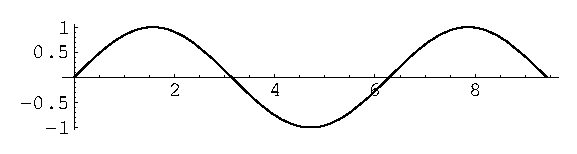
\includegraphics[width=8.5cm]{image1}}
% 		%  \vspace{2.0cm}
% 		\centerline{(a) Result 1}\medskip
% 	\end{minipage}
% 	%
% 	\begin{minipage}[b]{.48\linewidth}
% 		\centering
% 		\centerline{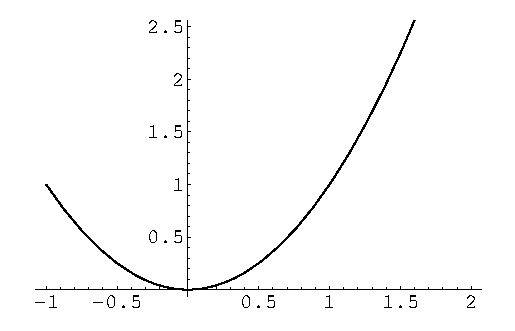
\includegraphics[width=4.0cm]{image3}}
% 		%  \vspace{1.5cm}
% 		\centerline{(b) Results 2}\medskip
% 	\end{minipage}
% 	\hfill
% 	\begin{minipage}[b]{0.48\linewidth}
% 		\centering
% 		\centerline{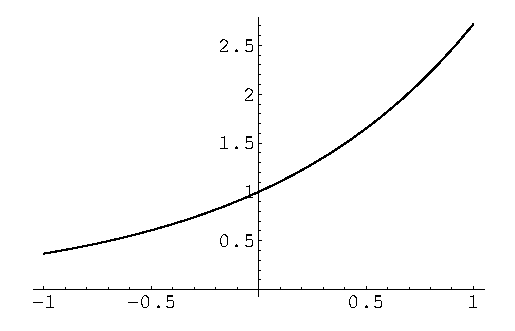
\includegraphics[width=4.0cm]{image4}}
% 		%  \vspace{1.5cm}
% 		\centerline{(c) Result 3}\medskip
% 	\end{minipage}
% 	%
% 	\caption{Example of placing a figure with results.}
% 	\label{fig:example}
% 	%
% \end{figure}

% References should be produced using the bibtex program from suitable
% BiBTeX files (here: strings, refs, manuals). The IEEEbib.bst bibliography
% style file from IEEE produces unsorted bibliography list.
% -------------------------------------------------------------------------
% \bibliographystyle{IEEEbib}
% \bibliography{refs}

\end{document}